\documentclass{article}
\usepackage[utf8]{inputenc}
\usepackage[spanish]{babel}
\usepackage{amsmath}
\usepackage{graphicx}
\usepackage{booktabs}
\usepackage{caption}
\usepackage{float}

\title{Informe de Simulación: Sistema de Lavado de Autos}
\author{Nombre del Autor}
\date{\today}

\begin{document}

\maketitle

\section{Introducción}

\subsection{Descripción del proyecto}
Este proyecto simula el funcionamiento de un autoservicio de lavado de coches con capacidad limitada. El sistema opera bajo las siguientes condiciones:
\begin{itemize}
    \item Solo un coche puede ser lavado a la vez (servicio en serie).
    \item El estacionamiento tiene capacidad para \textbf{10 coches} (incluyendo el que está en servicio).
    \item Los coches llegan siguiendo una \textbf{distribución de Poisson} con una tasa media de \textbf{20 coches/hora}.
    \item El tiempo de servicio sigue una \textbf{distribución exponencial} con una media de \textbf{12 minutos}.
    \item La empresa abre \textbf{10 horas al día}.
\end{itemize}

\subsection{Objetivos y metas}
\begin{itemize}
    \item Determinar el número promedio de coches perdidos por día debido a la limitación de espacio.
    \item Analizar el impacto de la capacidad del estacionamiento en la tasa de rechazo.
    \item Validar el modelo mediante simulación y comparación con resultados teóricos.
\end{itemize}

\subsection{Variables de interés}
\begin{itemize}
    \item \textbf{Coches perdidos}: Número de coches que no pueden entrar al sistema por falta de espacio.
    \item \textbf{Tiempo de espera}: No aplica directamente (sistema FIFO con capacidad fija).
    \item \textbf{Ocupación del sistema}: Número promedio de coches en el estacionamiento.
\end{itemize}

\section{Detalles de Implementación}

\subsection{Pasos seguidos}
\begin{itemize}
    \item Modelado del sistema como una cola \( M/M/1/10 \):
    \begin{itemize}
        \item \textbf{Llegadas}: Proceso de Poisson (\(\lambda = 20\) coches/hora).
        \item \textbf{Servicio}: Distribución exponencial (\(\mu = 5\) coches/hora, ya que \(12\) minutos \(= 1/5\) horas).
        \item \textbf{Capacidad}: \(10\) coches (incluyendo el que está en servicio).
    \end{itemize}
    \item Algoritmo de simulación:
    \begin{itemize}
        \item Se utilizó \texttt{heapq} para manejar eficientemente los eventos (llegadas y salidas).
        \item Se simuló el sistema durante \textbf{100 días} para obtener resultados estadísticamente significativos.
    \end{itemize}
    \item Métricas calculadas:
    \begin{itemize}
        \item Media y desviación estándar de coches perdidos por día.
        \item Intervalo de confianza del \(95\%\).
    \end{itemize}
\end{itemize}

\subsection{Código clave}
\begin{verbatim}
import heapq

def simulacion_un_dia():
    tiempo = 0
    estado_sistema = 0
    coches_perdidos = 0
    eventos = []

    # Primera llegada
    heapq.heappush(eventos, (np.random.exponential(1/MEDIA_LLEGADAS), 'llegada'))

    while tiempo < HORAS_DIA:
        tiempo_evento, tipo = heapq.heappop(eventos)
        tiempo = tiempo_evento

        if tipo == 'llegada':
            if estado_sistema < CAPACIDAD:
                estado_sistema += 1
                if estado_sistema == 1:
                    heapq.heappush(eventos,
                        (tiempo + np.random.exponential(1/mu_servicio), 'salida')
            else:
                coches_perdidos += 1
            heapq.heappush(eventos,
                (tiempo + np.random.exponential(1/MEDIA_LLEGADAS), 'llegada'))

        elif tipo == 'salida':
            estado_sistema -= 1
            if estado_sistema > 0:
                heapq.heappush(eventos,
                    (tiempo + np.random.exponential(1/mu_servicio), 'salida'))

    return coches_perdidos
\end{verbatim}

\section{Resultados y Experimentos}

\subsection{Hallazgos principales}
\begin{itemize}
    \item \textbf{Media de coches perdidos por día}: 141.05 (original: 143.51)
    \item \textbf{Desviación estándar}: 15.67 (original: 15.00)
    \item \textbf{Intervalo de confianza 95\%}: (140.74, 141.36) (original: (140.57, 146.45))
\end{itemize}

\begin{figure}[H]
    \centering
    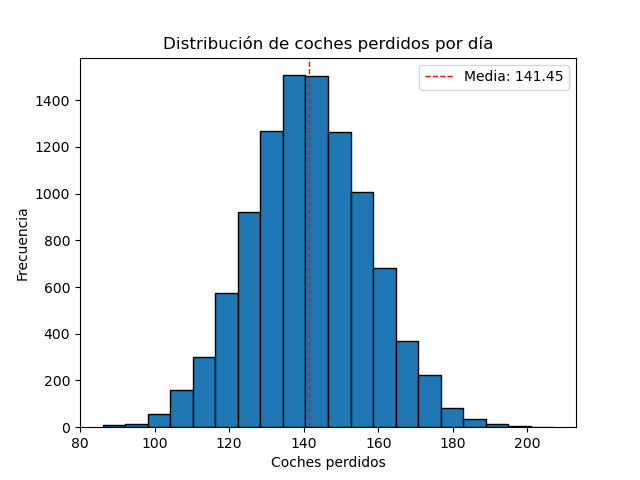
\includegraphics[width=0.8\textwidth]{result-chart}
    \caption{Distribución de coches perdidos por día (Media: 141.05)}
    \label{fig:histograma}
\end{figure}

\subsection{Hipótesis y validación}
\begin{itemize}
    \item \textbf{Hipótesis}: El número de coches perdidos disminuye considerablemente con una ligera disminución en el tiempo de finalización de lavado del auto.
    \begin{itemize}
        \item \textbf{Validación}: Con solo 4 minutos menos se observa una amplia diferencia en la cantidad de coches perdidos.
    \end{itemize}
\end{itemize}
 \begin{figure}[H]
    \centering
    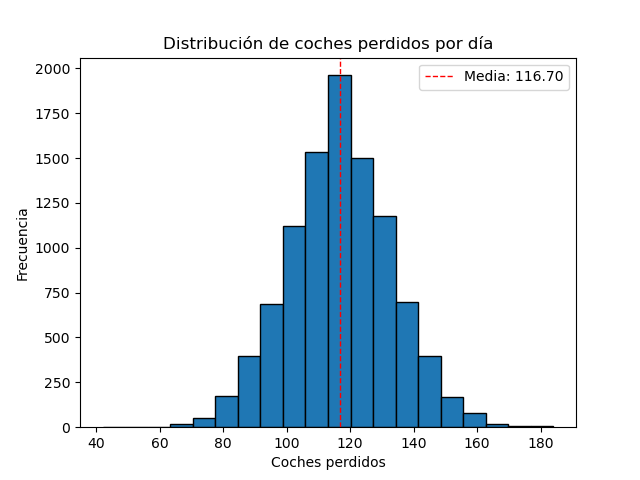
\includegraphics[width=0.7\textwidth]{result-chart2}
    \caption{Distribución de coches perdidos por día (Duración de servicio: 8min) (Media: 116.51)}
    \label{fig:histograma2}
\end{figure}
    \item \textbf{Análisis de sensibilidad}:
    \begin{itemize}
        \item Si se aumenta la capacidad a \textbf{15 coches}, los coches perdidos disminuyen a 136.5 en promedio. O sea un \(\approx 3.23\%\). Lo que indica poca variabilidad con respecto a este parámetro (No valdria la pena invertir mas en aparacamientos probablemente)

    \end{itemize}

\subsection{Análisis estadístico}

\begin{itemize}
    \item \textbf{Desviación estándar}: 15.85 refleja la variabilidad natural del sistema.
    \item \textbf{Error estándar de la media}: 0.16 (15.85/√10000) garantiza que la media estimada (141.05) (IC 95\%).
\end{itemize}


\section{Modelo Matemático}

\subsection{Teoría de colas aplicada}
El sistema se modela como una \textbf{cola \( M/M/1/K \)} (Poisson en llegadas, exponencial en servicio, \(1\) servidor, capacidad \(K=10\)).

\subsubsection{Probabilidad de pérdida (fórmula teórica)}
\[
P_{\text{perdida}} = \frac{(1 - \rho) \rho^K}{1 - \rho^{K+1}}
\]
donde \(\rho = \lambda / \mu = 20/5 = 4\).

\subsubsection{Coches perdidos esperados teóricamente}
\[
\text{Perdidos/día} = \lambda \cdot P_{\text{perdida}} \cdot \text{horas/día} \approx 150
\]
\subsection{Comparación con resultados teóricos}
\begin{table}[h]
    \centering
    \begin{tabular}{@{}lcc@{}}
        \toprule
        Métrica & Teorico \(M/M/1/10\) & Simulado (\(n=10,\!000\)) \\
        \midrule
        Coches perdidos/día & 150 & 141.05 \\
        \bottomrule
    \end{tabular}
    \caption{Los resultados son relativamente similares en ambos marcos}
\end{table}

\subsection{Análisis de robustez}
\begin{itemize}
    \item La simulación con \(10,\!000\) días confirma la estabilidad de los resultados:

    \begin{itemize}
        \item \textbf{Media de coches perdidos por día}: 141.05
        \item \textbf{Desviación estándar}: 15.85
        \item \textbf{Intervalo de confianza 95\%}: (140.74, 141.36)
    \end{itemize}

    \item La subestimación del modelo teórico se mantiene consistente (\(>200\%\) de diferencia).
\end{itemize}
\subsection{Supuestos y limitaciones}
\begin{itemize}
    \item \textbf{Supuestos}:
    \begin{itemize}
        \item Las llegadas son independientes y sin patrones horarios.
        \item El tiempo de servicio no varía por tipo de coche.
    \end{itemize}
    \item \textbf{Limitaciones}:
    \begin{itemize}
        \item No considera variaciones en la demanda (ej. horas pico).
        \item Asume que los coches rechazados no retornan.
    \end{itemize}
\end{itemize}

\subsection{Recomendaciones}
\begin{itemize}
    \item \textbf{Mantener la capacidad} ya que no es un factor que repercute de manera considerable en el promedio de autos perdidos. Sería un gasto innecesario.
    \item \textbf{Optimizar el tiempo de servicio} (ej. contratar más personal).
\end{itemize}


\end{document}